
Provided with a membership protocol capable of coordinating nodes into building an efficient tree structure, we now discuss how we leveraged it to provide efficient abstractions for performing aggregation/collection of metrics about the execution of nodes (or services) executing in the system in a decentralized manner. In this section, we cover the three implemented aggregation primitives: (1) tree aggregation, (2) neighbourhood aggregation, and (3) global aggregation, starting with tree aggregation.

\subsection{Tree aggregation} \label{sec:mon_protocol:tree_agg}

Tree aggregation is a mechanism that embeds an \textbf{aggregation tree} into the overlay protocols' to collect an aggregated value for all nodes which are descendants of the node performing this mechanism (also denoted the \textbf{root of the aggregation tree}). This mechanism can be performed by any node in the system, and if two different nodes are aggregating the same values and a node is a descendant of the other, then the descendant node will (when possible) reuse the values of the already existing aggregation tree by embedding its tree into the ascendants'.

The pseudocode for this mechanism can is provided in Algorithm \ref{alg:mon:tree_agg}. The first lines define the necessary state to execute this aggregation mechanism (line \ref{alg:mon:tree_agg:state}), starting by the active view, composed by: the parent, children, and siblings of the node (maintained by the overlay protocol with changes to it propagated through notifications). In addition, the state also contains three maps, the first map, called ``tIds'', contains the necessary metadata for each aggregation tree. Each value of this map is composed of: (1) the height of the tree, (2) the merge function, (3) the query to generate local values, (4) the periodicity to export values, (5) the output metric name, (6) the ID of the corresponding timer, (6) a boolean value representing if the value should be exported locally, (7) a boolean representing if the parent is also in the tree (and the node must propagate values to it or not), and finally, (8) the ID of the tree from the parent's perspective (or nil, if the node has no parent). The second map (denominated ``lastSeen'') contains a timestamp for each tree, representing the last time the parent has sent a message refreshing the existence for that tree. Finally, the ``childValues'' map contains, for each tree, the values emitted by the children and the timestamp of their reception.

\begin{algorithm}
\caption{Tree aggregation} \label{alg:mon:tree_agg}
\begin{algorithmic}[1]

    \asdstate \label{alg:mon:tree_agg:state}
        \State parent,children,siblings \Comment{Defined by the overlay protocol}
        \State tIds \asdassign map()
        \State timerIds \asdassign map()
        \State lastSeen \asdassign map()
        \State childValues \asdassign map()
    \asdend

    \asdupon[StartTreeAggregationRequest(tHeight, mergeF, query, periodicity ,outmName)] 
    \label{alg:mon:tree_agg:start_req}
        \State tId \asdassign hash(tHeight + mergeF + query + periodicity + outmName) \label{alg:mon:tree_agg:start_req_start}
        \If{tId in tIds} 
            \State <tHeight, mergeF, query, periodicity, outmName, isLocal, isParentSub, ptId> \asdassign tIds[tId]
            \State tIds[tId] \asdassign <tHeight, mergeF, query, periodicity, outmName, true, isParentSub, ptId>
        \Else:
        \State tIds[tId] \asdassign <tHeight, mergeF, query, periodicity, outmName, true, false, nil>
        \State timerID \asdassign registerPeriodicTimer(ExportTreeAggTimer(tID), periodicity)
        \State timerIds[tId] \asdassign timerID
        \EndIf\label{alg:mon:tree_agg:start_req_end}
    \asdend

    \asdupon[ExportTreeAggTimer(tId)] \label{alg:mon:tree_agg:export_trigger}
        \State <tHeight, mergeF, query, periodicity, outmName, isLocal, isParentSub, ptId> \asdassign tIds[tId]
        \If{!isLocal }
            \If{timeSince(tIdLastSeen[tId]) > config.treeAggExpiration}
                \State tIds.delete(tId)
                \State lastSeen.delete(tId)
                \State cancelTimer(timerIds[tId])
                \State return
            \EndIf
        \EndIf
        \State res \asdassign aggregateValues(mergeF, resolveQuery(query), childValues[tID])
        \If{isLocal}
            \State storeLocalVal(res, outmName)
        \EndIf 
        \If{isParentSub}
            \State sendMessage(PropagateTAggValues<ptId, res>, parent)
        \EndIf
    \asdend

    \asdupon[receive(PropagateTAggValues<tID, res>, sender)] \label{alg:mon:tree_agg:recv_propag_vals}
        \If{tId in tIds and sender in children}
            \If{tID not in localValues}
                \State localValues[tID] = map()
            \EndIf
            \State localValues[tID][sender] = res
        \EndIf
    \asdend

    \asdrepeateveryx{config.PropagateTAggTimeout seconds} \label{alg:mon:tree_agg:propag}
        \State toSendArr \asdassign set 
        \For{tID in tids}
            \State <tHeight, mergeF, query, periodicity, outmName, isLocal, isParentSub, ptId> \asdassign tIds[tId]
            \If{isLocal \&\& tHeight > 0 || tHeight == -1}
                \State toSendArr.append(<max(tHeight -1, -1), mergeF, query, periodicity ,outmName, tID>)
            \EndIf
        \EndFor
        \For{c in chilren}        
            \State sendMessage(RefreshTreeAggFunc<toSendArr>, c)
        \EndFor
    \asdend

    \asdupon[receive(RefreshTreeAggFunc<tAggs>, sender)] \label{alg:mon:tree_agg:propag_recv}
        \If{parent == sender}
            \State toSendArr \asdassign set 
            \For{<tHeight, mergeF, query, periodicity, outmName, ptId> in tAggs}
                \State tId \asdassign hash(tHeight + mergeF + query + periodicity + outmName)
                \If{id in tIds}
                    \State <tHeight, mergeF, query, periodicity, outmName, isLocal, isParentSub, ptId> \asdassign tIds[tId]
                    \State lastSeen[id] \asdassign time.Now()
                    \State tIds[tId] \asdassign <tHeight, mergeF, query, periodicity, outmName, isLocal, true, ptId>
                    \If{!isLocal}
                        \State toSendArr.append(<max(tHeight -1, -1), mergeF, query, periodicity ,outmName, tID>)
                    \EndIf
                \Else
                    \State toSendArr.append(<max(tHeight -1, -1), mergeF, query, periodicity ,outmName, tID>)
                    \State tIds[tId] \asdassign <tHeight, mergeF, query, periodicity, outmName, false, true, ptId>
                    \State registerPeriodicTimer(HandleTreeAggTimer(tID), periodicity)
                \EndIf
            \EndFor
            \For{c in chilren}        
                \State sendMessage(RefreshTreeAggFunc<toSendArr>, c)
            \EndFor
        \EndIf
    \asdend

    \end{algorithmic}
\end{algorithm}
    

Nodes begin executing this mechanism whenever the API sends a ``StartTreeAggregationRequest'' request to the protocol, which contains the maximum height of the tree, the merge function, the query to obtain the local value, the periodicity at which to execute the aggregation procedure, and the resulting metric name. Upon the reception of this request (line \ref{alg:mon:tree_agg:start_req}), the node creates the ID for the aggregation tree by hashing the concatenation of: (1) the tree height, (2) the merge function, (3) the query, (4) the mechanism periodicity, and (5) the resulting metric name. By using this combination of parameters for the hash, nodes guarantee that aggregation trees with the same height (from the hashing nodes' perspective) have the same ID. Whenever two trees have the same ID, the node that detects this may reuse the already existing trees' aggregation results, thus not increasing the necessary messages to collect the metric values.
 
 After this, the node adds the tree ID to its local aggregation ``tIds'' map, first checking if there was already an existing tree with the same ID (meaning it may reuse the existing tree for obtaining the requested values). If there is, then it sets a flag signalling it should also save the values for that tree locally. Otherwise, it adds a new entry to the ``tIds'' map and sets up a periodic timer for that aggregation tree (lines \ref{alg:mon:tree_agg:start_req_start}-\ref{alg:mon:tree_agg:start_req_end}).

In order to federate nodes into their aggregation trees, nodes periodically (using configured intervals) broadcast to their children a ``Subscription'' message containing the metadata (including the ID) of the aggregation trees they are the root of (line \ref{alg:mon:tree_agg:propag}). Whenever this message is received (line \ref{alg:mon:tree_agg:propag_recv}), for each received ID, if it was previously present in the ``tIds'' map, the child marks the parent as a subscriber to that tree, and refreshes the timestamp associated with the tree in the ``LastSeen'' map. Conversely, for each received aggregation tree that was not previously in the ``tIds'' map, it sets a new periodic timer called ``ExportTreeAggTimer'', and adds the ID to the ``tIds'' map along with the tree metadata. Lastly, the node subtracts by one each of the received tree TTLs and sends a ``Subscription'' containing the ones with TTL higher than zero (or equal to -1) to its children. This means that if a tree has a single root node, and that node crashes or stops propagating ``Subscription'' messages, all other nodes belonging to that tree will stop sending any more ``Subscription'' messages.

Whenever the aforementioned periodic timer called ``ExportTreeAggTimer'' triggers for a certain aggregation tree, (line \ref{alg:mon:tree_agg:export_trigger}), the node checks if it has expired (i.e. if the parent stopped refreshing the tree), if it has, and the node is not a root of that tree, then it cancels the timer and deletes any related metadata. Conversely, if the node is a root of the tree, it sets the flag representing whether the node should propagate to the parent as ``false''. If the tree has not expired, the node evaluates the trees' query (this procedure will be explained in further detail in Section \ref{sec:mon_module}), obtaining its local value and merging it (using the supplied aggregation function) with all the values sent by its children, producing the final aggregated result (before merging the values, the node excludes all values with a timestamp older than a configurable duration).  Afterwards, if the node is a root of the tree, it stores the value locally, and if the flag signalling it should propagate to the parent has the value ``true'', it sends a ``PropagateTAggValues'' message to the parent containing the obtained value. Upon the reception of this ``PropagateTAggValues'' message by the parent, (line \ref{alg:mon:tree_agg:recv_propag_vals}), it verifies if it has the corresponding aggregation tree in its local ``tIds'' map, discarding the message if it is not present, and, stores the received value into its ``childValues'' map.

Although it is omitted from the pseudocode, it is essential to mention that for nodes that are roots of the aggregation trees, it is also possible (according to a configuration parameter) to store the neighbours' values locally (without merging with the local or any other neighbours' values). We believe this feature is useful for resource management applications, for example, in the case of an application that needs to deploy service replicas according to geographical proximity to a certain target, this feature can be useful for obtaining a histogram of latitudes and longitudes for all nodes ``behind'' a certain node in the active view. Using this information, a resource management application can have a sense of which direction to send messages to in order to find nodes located in a given geographical region (by recursively sending messages to nodes in the active view that have frequencies closer to the desired geographical region).

\subsection{Neighborhood aggregation} \label{sec:mon_protocol:neigh_agg}

Neighbourhood aggregation is the mechanism responsible for collecting metrics from neighbouring nodes. This feature is useful in resource management scenarios such as: whenever a node needs to perform service replication/migration, it may collect metrics related to the capacity and resource consumption of nearby nodes (in terms of hop distance) and evaluate which peer is the best candidate before performing such actions. 

In essence, this mechanism behaves similarly to a hop-based Pub-Sub system. Although the designated name for this protocol is neighbourhood aggregation, the nodes actually do not perform aggregation of the values. Instead, nodes collect all the values provided by their nodes within a (configurable) hop range. Similarly to tree aggregation (Section \ref{sec:mon_protocol:tree_agg}), a node performing this mechanism creates an aggregation tree rooted on itself by broadcasting ``Subscription'' messages periodically with a configurable hop-based range (or TTL) for all its neighbours. Nodes that receive this message become federated in the aggregation tree, decrease the message TTL, and if the TTL is more than zero, and rebroadcast it to peers in the active view in a way that creates an acyclical graph. Afterwards, for each tree, all federated nodes periodically propagate their locally obtained values (from evaluating the supplied query) towards the root of each tree using the reverse path established by the ``Subscription'' messages. 

Trees have associated IDs, generated using hashing in a similar manner to the tree algorithm defined in Section \ref{sec:mon_protocol:tree_agg} (without using the level in the hash process), and consequently, all nodes collecting the values from the same query using this mechanism will have trees with equal IDs. Nodes belonging to overlapping trees (i.e. in the hop range of two different nodes collecting values in this manner) only generate values periodically for one of the trees and propagate the generated value towards the direction of the multiple tree roots, preventing unnecessary query evaluations. In addition, nodes in overlapping trees, when possible, also deduplicate the ``Subscription'' messages (maintaining the federation of these trees).

This mechanism, similarly to Tree Aggregation (Section \ref{sec:mon_protocol:tree_agg}), is triggered via a request from the API containing, among other parameters, the query to obtain the local values, the hop range, and the target periodicity to collect the values. The receiver of the request, denoted the \textbf{root of the aggregation tree},(illustrated by node A in Figure~\ref{fig:mon_protocol:img:neigh_agg_sub}) creates the ID for that aggregation tree by hashing a combination of the metric name and the periodicity. This process makes nodes with equal parameters have equal IDs and become federated to the same tree. After the ID generation, the node begins propagating a ``Subscription'' message periodically to its immediate neighbours (illustrated in step 2 of Figure~\ref{fig:mon_protocol:img:neigh_agg_sub}) containing the ID of the tree, the TTL, the query to obtain their local values, and the mechanism periodicity. 

\begin{figure}[htbp]
    \centering
    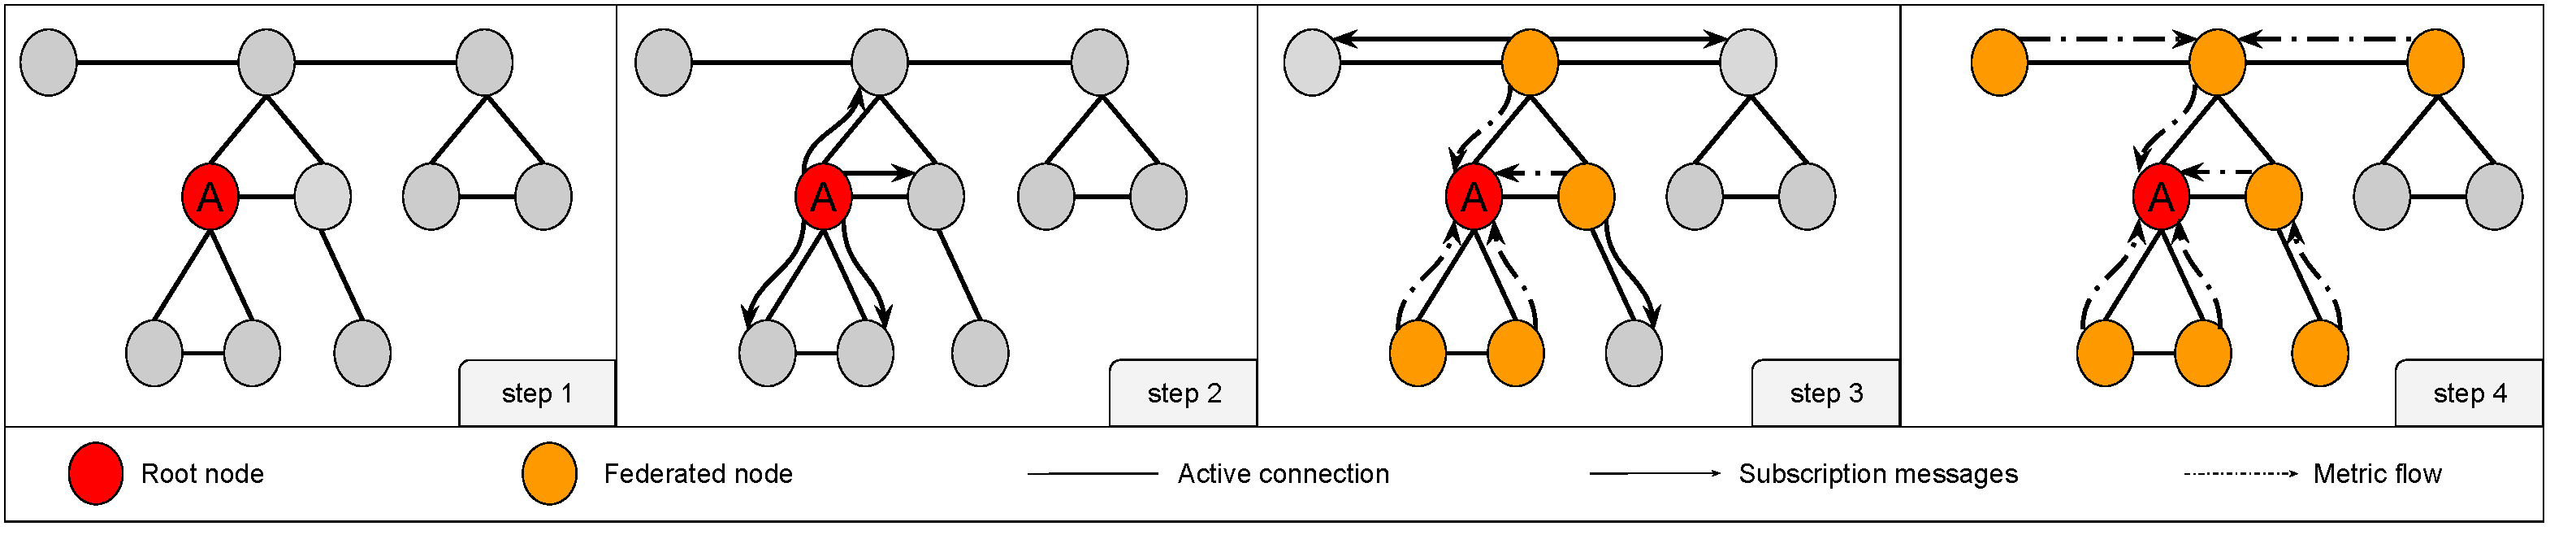
\includegraphics[width=\textwidth]{Chapters/aggregation/images/neigh-agg-subscribe.pdf}
    \caption{Neighborhood aggregation subscription process (TTL=2)}
    \label{fig:mon_protocol:img:neigh_agg_sub}
\end{figure}
     
Whenever a node receives this ``Subscription'' message, it performs the following steps:

\begin{enumerate} \label{sec:mon_protocol:enum:neigh_agg_sub_opts}
    \item Verifies the message came from a node contained in the active view, if it did not, the message is discarded.
    \item Stores, for that sender, the ID of the tree, the TTL of the message and a timestamp of the current time. If there is already such an entry, instead, its timestamp is refreshed.
    \item Decreases the TTL of the message by one.
    \item If the message TTL is 0, the node returns from this procedure.
    \item Following, the node performs the following steps to decide where to broadcast to:
            \begin{enumerate}
                \item If the message came from a parent or a sibling, the node broadcasts the message to its children.
                \item If it came from a child, then the node broadcasts the message to the parent and its siblings.
                \item Before broadcasting to any node, the sender verifies if it has sent a ``Subscription'' message with a higher or equal TTL than the TTL from the received one to these nodes in the last (configurable) time window. If it has, the sender skips the message emission for that node.
            \end{enumerate}
\end{enumerate}

With this, in case two different nodes in the system are collecting the same metrics and using the same periodicity, the ``Subscription'' messages are not sent unnecessarily to nodes already subscribed to that tree. This process is illustrated by node ``A'' in Figure~\ref{fig:mon_protocol:img:neigh_agg_second_sub}, where it receives the ``Subscribe'' message and does not propagate it to its siblings nor parent, as it is already federated to the tree (rooted on itself with TTL= 2) and has sent a ``Subscription'' message to its siblings and parent in the previous step.

\begin{figure}[htbp]
    \centering
    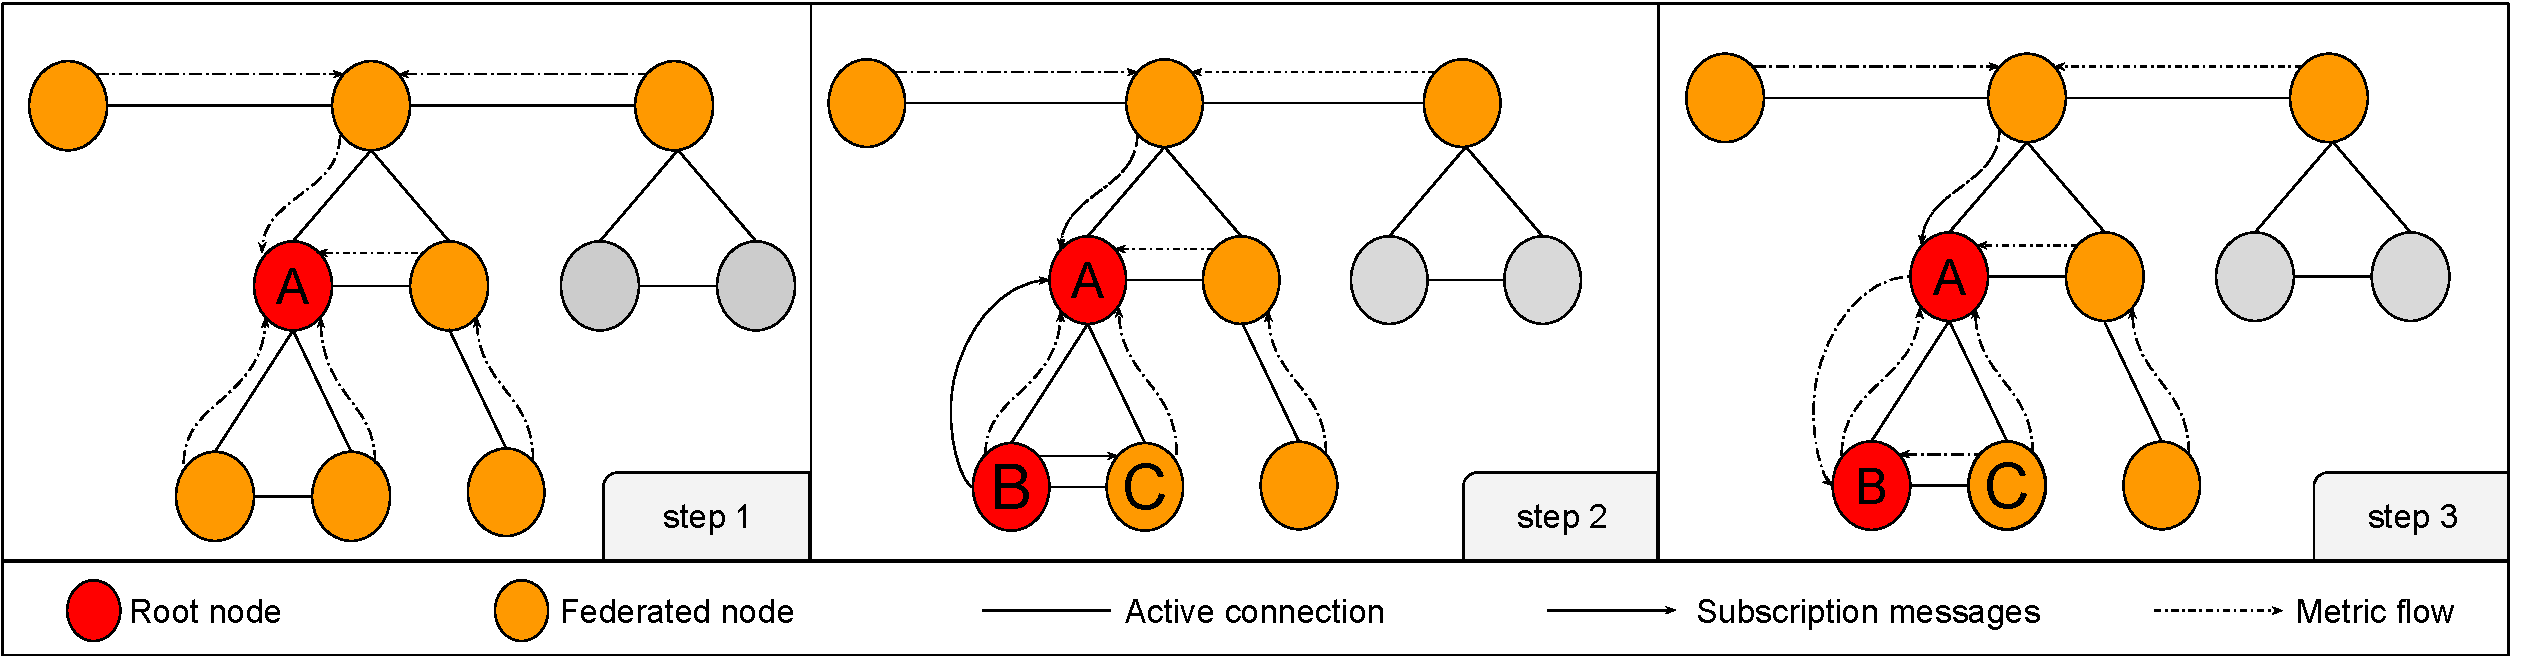
\includegraphics[width=\textwidth]{Chapters/aggregation/images/2nd_subscribe.pdf}
    \caption{Neighborhood aggregation second subscribe (TTL=2)}
    \label{fig:mon_protocol:img:neigh_agg_second_sub}
\end{figure}


\begin{figure}[htbp]
    \centering
    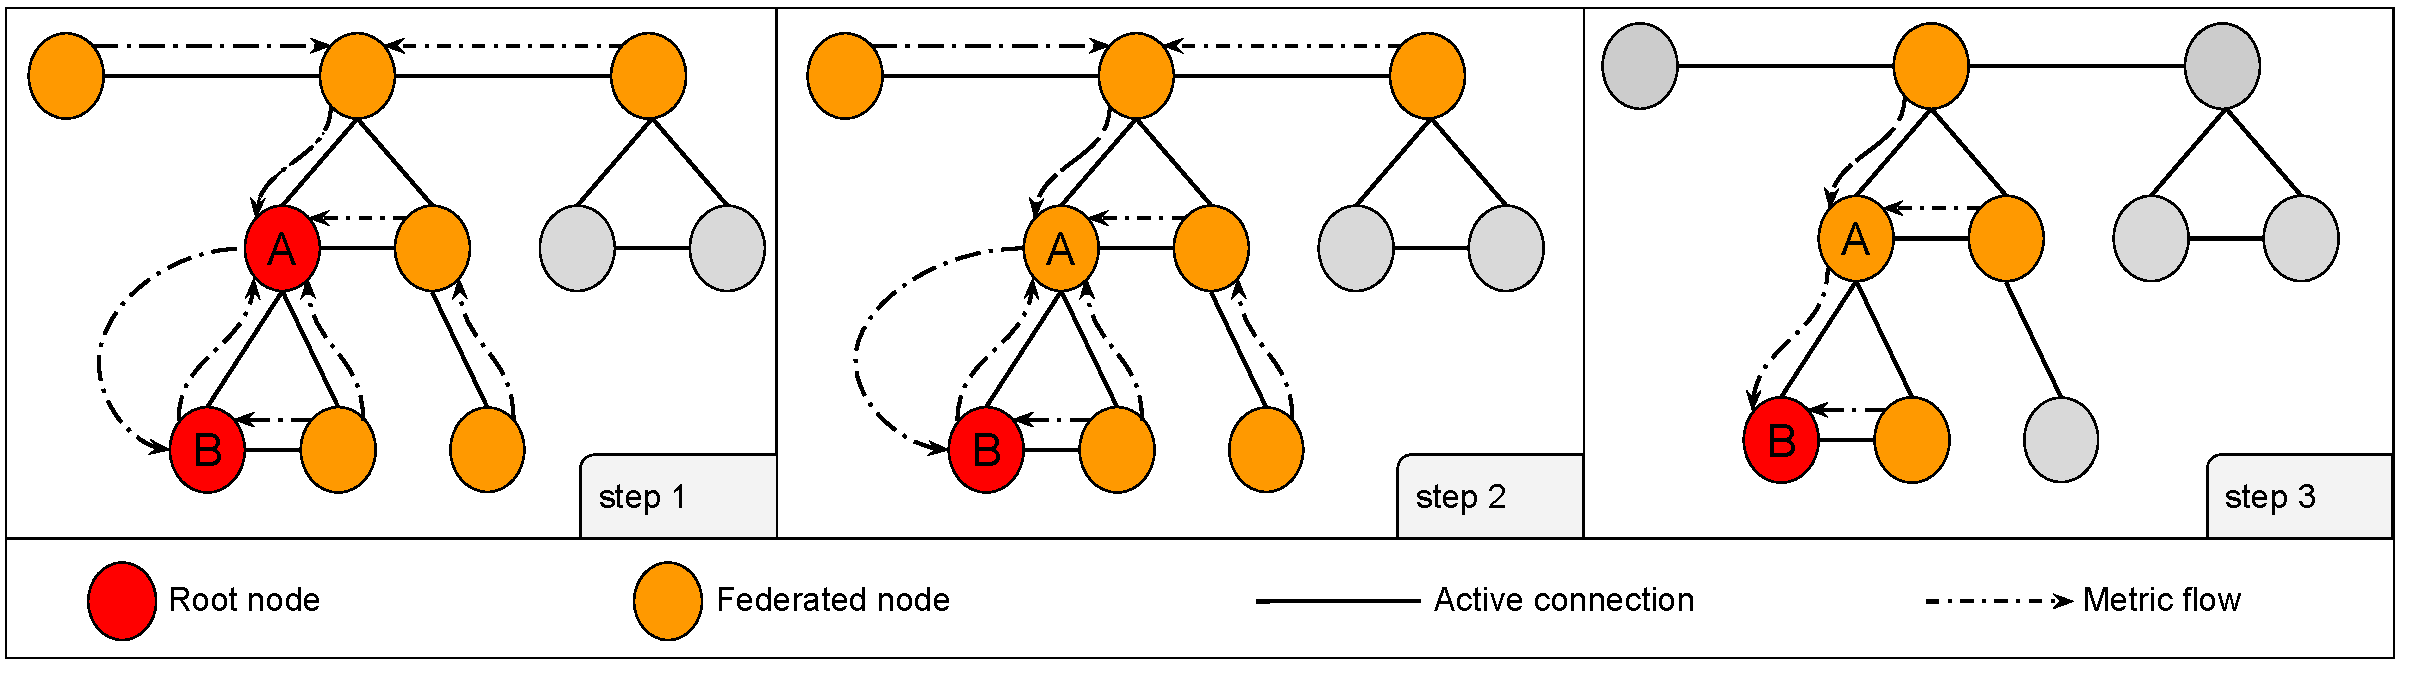
\includegraphics[width=\textwidth]{Chapters/aggregation/images/unsubscribe_process.pdf}
    \caption{Neighborhood unsubscribe (TTL=2)}
    \label{fig:mon_protocol:img:neigh_agg_unsub}
\end{figure}

After nodes become federated in the trees, they begin to periodically evaluate the supplied query and obtain their local metric values (storing them locally if they are a root of that tree). When a node obtains its local metric value, it propagates a message containing the metric value and a hop counter to every other node in its active view that has sent a ``Subscription'' message within a configurable time frame with a TTL lower or equal than the messages'. Nodes that receive the propagation of these values increase the hop counter and repeat this process. This process is illustrated in Figures~\ref{fig:mon_protocol:img:neigh_agg_sub} \ref{fig:mon_protocol:img:neigh_agg_second_sub} and~\ref{fig:mon_protocol:img:neigh_agg_unsub}. 
    
Lastly, nodes periodically verify, for each tree, the time passed since the reception of the last ``Subscribe'' message. If it exceeds a configurable time frame, the entry is removed, and that node will stop receiving the propagation of metric values. When nodes remove the expired entry, if there is no other entry for that tree ID and the node is not a root of that tree, they delete all metadata related to that tree and stop propagating metric values (illustrated in Figure~\ref{fig:mon_protocol:img:neigh_agg_unsub}).

\subsection{Global aggregation} \label{sec:mon_protocol:global_agg}

Global aggregation is the mechanism executed whenever a certain client wishes to obtain a summarized global view of the system (e.g. the total number of nodes in the system). This process, similarly to the ones described in Sections \ref{sec:mon_protocol:tree_agg} and \ref{sec:mon_protocol:neigh_agg}, is started via a request from the API and functions by federating nodes of the system into \textbf{aggregation trees}, rooted on the nodes that are collecting the aggregate values. In global aggregation, all nodes participate in all aggregation trees, either as a root (if they wish to collect the globally aggregated value), or alternatively as aggregator nodes. Additionally, if a tree has multiple root nodes, then nodes, when possible, reuse the metric values from the first tree root towards the other roots, and deduplicate the maintenance mechanisms of the aggregator trees. 

This mechanism is inspired in the work from Mirage protocol \cite{akosThesis}, which employs an aggregation technique that leverages a tree-shaped overlay to allow the computation of a globally aggregated value in a decentralized and efficient manner by every node in the system. This is achieved by having every node periodically broadcasting to every neighbouring peer their aggregated value minus the neighbours' contribution. Nodes that receive this broadcast merge all received contributions with the locally generated one. The continuous execution of this procedure results in all nodes obtaining the global aggregated value without resorting to aggregating the values toward a single node in the system.

% Nodes federated in these trees that are not the roots are denoted \textbf{aggregator} nodes, and their role within this mechanism is to collect their neighbours' metric values, aggregate them, and send them toward the root of the tree.

In this mechanism, we leverage the same aggregation technique to collect globally aggregated values in multiple (but not necessarily all) nodes of the system in a decentralized manner. However, unlike the original Mirage protocol, instead of only performing aggregation of a single metric value, we generalize the approach to allow the on-demand creation and teardown of aggregation trees, rooted in one or more nodes, with all roots collecting the globally aggregated value in a decentralized manner. The relaxation of these constraints creates additional challenges regarding the transmission of redundant messages to maintain the multiple aggregation trees and the decommissioning of the trees, which we attempt to solve in this work. It is important to mention that, in a scenario where all nodes of the system are roots of the aggregation tree, this mechanism behaves similarly to the originally proposed in \cite{akosThesis}, with the only difference being of allowing the on-demand start and decommission of the aggregation process.

\begin{algorithm}
    \caption{Global aggregation} \label{alg:mon:global_agg}
    \begin{algorithmic}[1]

    \asdstate \label{alg:mon:global_agg:state_start}
        \State parent : Node \Comment{Defined by the overlay protocol} 
        \State children : dict<string,Node> \Comment{Defined by the overlay protocol} 
        \State siblings : dict<string,Node> \Comment{Defined by the overlay protocol}  
        \State lastTimeSent : dict<string, dict<string, timeStamp>> \asdassign dict()
        \State neighValues : dict<string, dict<value, timeStamp>> \asdassign dict() \label{alg:mon:global_agg:state_end}
        \State tIds : dict<string, <string, string, timeDuration, string, string, boolean, dict< string, timeStamp>> \asdassign dict()
    \asdend

    \asdupon[StartGlobalAggregationRequest(diffF, mergeF, query, periodicity ,outmName)] 
    \label{alg:mon:global_agg:start_req}
        \State tId \asdassign hash(diffF + mergeF + query + periodicity) 
        \If{tId in tIds} 
            \State <diffF, mergeF, query, periodicity, outmName, timerId, isLocal, aggNeighs> \asdassign tIds[tId]
            \State tIds[tId] \asdassign <mergeF, query, periodicity, outmName, timerId, true, aggNeighs>
        \Else
            \State timerID \asdassign registerPeriodicTimer(ExportGlobalAggTimer(tId), periodicity)
            \State tIds[tId] \asdassign <mergeF, query, periodicity, outmName, timerId, true, dict()>
            \State neighValues[tId] = dict()
            \State
        \EndIf
    \asdend

    \asdrepeateveryx{config.PropagateGAggTimeout seconds} \label{alg:mon:global_agg:propag}
        \State toSendArr \asdassign set \label{alg:mon:global_agg:propag_start}
        \For{tId in tIds}
            \State <diffF, mergeF, query, periodicity, outmName, timerId, isLocal, aggNeighs> \asdassign tIds[tId]
            \For{<node, timestamp> in aggNeighs}
                \If{timeSince(timestamp) > config.SubExpirationDuration}
                    \State aggNeighs.remove(node)
                \EndIf
            \EndFor
            \If{aggNeighs.length == 0 \&\& !isLocal}
                \State tIds.remove(tId)
                \State continue
            \EndIf
            \If{isLocal}
                \State toSendArr \asdassign toSendArr + <diffF, mergeF, query, periodicity, outmName, tId>
            \EndIf
        \EndFor
        \State PropagateGAggTrees(toSendArr, parent + children) \label{alg:mon:global_agg:propag_end}
    \asdend

    \asdupon[receive(RefreshGaggTree<gAggs>, sender)] \label{alg:mon:global_agg:propag_recv}
        \State gAggTreeArr \asdassign set 
        \For{<diffF, mergeF, query, periodicity, outmName, tId> in gAggs}
            \If{id in tIds} \label{alg:mon:global_agg:propag_recv_merge}
                \State gAggTreeArr.append(<diffF, mergeF, query, periodicity ,outmName, timerId, tId>)
                \State neighValues[tId] = dict()
                \State tIds[tId] \asdassign <diffF, mergeF, query, periodicity ,outmName, timerId, false, <sender: time.Now()>>
                \State registerPeriodicTimer(HandleTreeAggTimer(tId), periodicity)
            \Else \label{alg:mon:global_agg:propag_recv_merge_end}
                \State <diffF, mergeF, query, periodicity ,outmName, timerId, isLocal, aggNeighs> \asdassign tIds[tId]
                \State aggNeighs[sender] \asdassign time.Now()
                \State tIds[tId] \asdassign <diffF, mergeF, query, periodicity ,outmName, timerId, isLocal, aggNeighs>
                \If{isLocal}
                    \State continue
                \EndIf
            \EndIf
        \EndFor
        \If{sender == parent}
            \State PropagateGAggTrees(gAggTreeArr, children)
        \EndIf
        \If{sender in children}
            \State PropagateGAggTrees(gAggTreeArr, children - sender + parent)
        \EndIf
    \asdend


    \asdupon[ExportGlobalAggTimer(tId)] \label{alg:mon:global_agg:export_trigger}
        \State <diffF, mergeF, query, periodicity, outmName, timerId, isLocal, aggNeighs> \asdassign tIds[tId] \label{alg:mon:global_agg:export_trigger_init_part}
        \State removeOldNeighValues(neighValues[tId])
        \State localVal \asdassign resolveQuery(query)
        \State res \asdassign evalFunc(mergeF, localVal, neighValues[tId])
        \If{isLocal}
            \State storeValLocally(res, outmName)
        \EndIf  \label{alg:mon:global_agg:export_trigger_init_part_end}
        \For{<node, timestamp> in aggNeighs}\label{alg:mon:global_agg:export_trigger_last_part}
            \State sendMessage(PropagateGAggValues<tId, evalFunc(diffF, res, neighValues[tId][node]>, node)
           
        \EndFor \label{alg:mon:global_agg:export_trigger_last_part_end}
    \asdend

    \asdupon[receive(PropagateGAggValues<tId, res>, sender)] \label{alg:mon:global_agg:recv_propag_vals}
        \If{tId in tIds and sender in children || sender == parent}
            \State neighValues[tId][sender] = res, time.Now()
        \EndIf
    \asdend

    \asdprocedure{PropagateGAggTrees(gAggTreeArr, nodeList)} \label{alg:mon:global_agg:propag_procedure}
        \For{node in nodeList}
            \State toSendToNode \asdassign set()
            \For{<diffF, mergeF, query, periodicity ,outmName, timerId, tId> in gAggTreeArr}
                \If{lastTimeSent[node][tId] == nil || time.Since(lastTimeSent[node][tId]) > config.RefreshMessageBackoff}
                    \State toSendToNode \asdassign toSendToNode + <diffF, mergeF, query, periodicity ,outmName, timerId, tId>
                \EndIf
            \EndFor
            \State lastTimeSent[node][tId] \asdassign time.Now()
            \State sendMessage(RefreshGaggTree<toSendToNode>,node)
        \EndFor
    \asdend

    \end{algorithmic}
\end{algorithm}
    

The state necessary for the execution of this mechanism (presented in Algorithm \ref{alg:mon:global_agg} lines \ref{alg:mon:global_agg:state_start} to \ref{alg:mon:global_agg:state_end}) starts with the active view of the node executing the mechanism, composed by the parent, children and siblings of the node in question. Changes in this view are propagated by notifications emitted by the overlay protocol (these are omitted from the pseudocode for readability). In addition, the state contains a map denominated ``lastTimeSent'' that contains for each tree ID, and for each neighbouring node, a timestamp corresponding to the last time that node has refreshed the existence of the tree with that ID. Additionally, each node also maintains a ``neighValues'' map, which stores, for each tree, the propagated neighbour values and a timestamp of the reception of these values. Finally, each node owns a map denominated ``tIds'',  which holds the metadata needed to manage the aggregation trees, composed by: (1) a difference function, used to remove the contributions of a certain node from an aggregated value, (2) the merge function, used for merging two or more values into an aggregated value, (3) the query to obtain the local values, (4) the resulting output name for the aggregated metric, (5) the periodicity at which to collect the aggregated value, (6) a boolean representing if the node executing the protocol is a root of the aggregation tree, and finally, (7) a map called ``aggNeighs'' which contains the peers that are interested in receiving values for that tree (previously referred to as the aggregator nodes).

This mechanism is initiated with the reception of a request from the API (line \ref{alg:mon:global_agg:start_req}), which contains multiple parameters: (1) the difference function, (2) the merge function, (3) the query to obtain the local value (4) the periodicity to perform this mechanism, and (5) the resulting metric name (to label the output values). Upon reception of this request, the node hashes the concatenation of the difference function, the merge function, the query, and the periodicity of the request, obtaining the tree ID, which will be common to every node in the tree. After the ID generation, the node checks if there already is a tree with that ID present in its local ``tIds'' map, setting as true the variable which denotes if the node should save the aggregated value locally. If there is no tree with such ID previously present, the node sets up a new ``ExportGlobalAggTimer'' with the provided periodicity and creates a new entry in the ``neighValues'' map for that tree.

As previously mentioned, global aggregation allows the on-demand creation and decommission of aggregation trees. This process is defined in alg. \ref{alg:mon:global_agg} lines \ref{alg:mon:global_agg:propag_start} to \ref{alg:mon:global_agg:propag_end}), where, as previously mentioned, nodes periodically send messages named ``RefreshGaggTree'' containing the aggregation trees they are the roots of to their children and parent and clear all entries in the ``aggNeighs'' that are older than a configured time frame. If a tree has no more entries in this map, and the ``isLocal'' flag is not set to true, then that tree is decommissioned.

% This process is achieved through a time-based mechanism, where nodes periodically refresh the trees they are the roots of via message broadcasts which are then forwarded by other nodes in the system until they reach every node. If an aggregator node (not a root) does not receive a message from any neighbour refreshing the existence of a tree within a certain time frame, it decommissions the tree locally. 

Whenever the ``RefreshGaggTree'' message is received (Algorithm \ref{alg:mon:global_agg} line \ref{alg:mon:global_agg:propag_recv}), the receiver adds the previously unknown trees into its local ``tIds'' map and sets up a periodic ``ExportGlobalAggTimer'' for each added tree (lines \ref{alg:mon:global_agg:propag_recv_merge} to \ref{alg:mon:global_agg:propag_recv_merge_end}). Alternatively, if the tree was previously in the ``tIds'' map, the node refreshes the sender's entry in the ``aggNeighs'' map. Finally, the node removes the trees present in the message where it is also a root of (deduplicating the tree maintenance mechanisms) and forwards the remaining trees to every node in its active view, excluding the sender. Before transmitting the trees to each node, the node checks, for each tree, if it has transmitted a ``RefreshGaggTree'' message containing the same tree in the last (configurable) time frame. If it has, then it does not propagate that tree to that node. These verifications are performed to prevent trees from being refreshed multiple times unnecessarily. 

\subsubsection{Metric propagation}

With the aggregation tree established, we now explain how the values are propagated and aggregated by each tree in the system. As previously mentioned, nodes set up an ``ExportGlobalAggTimer'' for each registered tree, whenever this timer triggers (alg.  \ref{alg:mon:global_agg} line \ref{alg:mon:global_agg:export_trigger}), the node first removes all out-of-date neighbour values for the corresponding tree (according to a configurable timeout) and evaluates the query, obtaining its local value. Then, using the neighbour values and the locally obtained value, it applies the merge function and obtains the globally aggregated value, which it stores locally if configured by the ``isLocal'' flag (lines \ref{alg:mon:global_agg:export_trigger_init_part} to \ref{alg:mon:global_agg:export_trigger_init_part_end}). Then, for each entry previously in the ``aggNeighs'' map, it sends a ``PropagateGAggValues'' message with the aggregated value minus the node's contribution and the tree ID. (lines \ref{alg:mon:global_agg:export_trigger_last_part} to \ref{alg:mon:global_agg:export_trigger_last_part_end}). 

Finally, whenever nodes receive the ``PropagateGAggValues'' message (alg. \ref{alg:mon:global_agg} line \ref{alg:mon:global_agg:export_trigger}) containing the aggregated value and the tree ID, they verify that it was sent from either the parent or the children and that the tree ID is in their local ``tIds'' map, discarding the message any one of these conditions is observed. Finally, they store the propagated value locally in their ``neighValues'' map for later use in computing the aggregated value.

In sum, nodes that are roots of their aggregation trees will, over time, receive aggregated values from their nodes, which are essentially sent and aggregated by all other nodes using the reverse path taken by the``RefreshGaggTree'' messages. Given the fact that nodes only use their parents and children of the tree topology to forward messages (thus ensuring the tree has no cycles, as there is only a single path from any node to each other node in the system), by propagating to a neighbour the resulting aggregated value without the effects of its contribution \cite{akosThesis}, multiple nodes in the system can simultaneously obtain the aggregated value efficiently and in a decentralized manner.

\subsection{Summary}

In this section, we presented the devised aggregation protocol. This protocol leverages the devised overlay protocol's tree structure to perform efficient propagation/aggregation of information in a decentralized manner. This protocol is coalesced by three decentralized information aggregation/collection primitives, which we believe to be useful for gathering partial or complete system information to perform decentralized resource management actions. 

The first primitive is \textbf{tree aggregation}, where nodes, when requested, form aggregation trees (with configurable range) rooted upon themselves. These trees extend only to their descendants in the original overlay protocol tree, and nodes federated in these trees periodically merge their local value with their childrens' and send a message containing it to their parents. In case one descendant is executing the same primitive with a tree with the same range (from the descendants' perspective), it simply reuses the parent's tree to obtain the intended aggregated value. 

The second primitive is \textbf{neighborhood aggregation}, where nodes collect, on-demand and in a decentralized manner, the metrics of nodes in a hop-defined range. This mechanism behaves similarly to a pub-sub system, where nodes periodically propagate messages which federate other nodes in trees rooted upon themselves. Nodes in these trees propagate their local values periodically using the reverse paths taken by the federation messages. In this primitive, nodes (when possible) deduplicate federation messages and multiplex metric propagations.

Lastly, the third primitive called \textbf{global aggregation} is a primitive where nodes collect and aggregate, also on-demand and in a decentralized manner, a value that corresponds to the globally aggregated value of the system. This primitive is inspired by work from the state-of-the-art, however, it relaxes constraints imposed by the original work, such as performing the mechanism with only a partial set of the nodes being tree roots, in addition to allowing the technique to be performed in an on-demand fashion (based on API requests).

We believe these primitives are useful for resource management decisions such as, for example, maintaining a proportion of replicas to nodes, by employing \textbf{tree aggregation} collecting all the descendants' number of replicas and number of nodes, the tree roots can, in a decentralized and independent manner, perform replication or decommission of replicas to maintain the target value. The same applies to \textbf{global aggregation}, which allows nodes to, for example, collect the total number of replicas in the system and perform replication actions if they reach a lower than configured number. Lastly, \textbf{neighbourhood aggregation} allows nodes to collect information about nearby nodes, which can also be used to improve system QOS by, for example, deploying a server closer to a client in terms of geographical distance.

It is important to mention that while in this work we present the protocol leveraging the overlay protocol defined in \ref{sec:overlay_network}, the protocol is agnostic to which overlay protocol is executing underneath it, as long as it has the following characteristics: (1) forms one or more tree-shaped networks, whose roots are interconnected; (2) Nodes in these trees must be connected to their parents, children and siblings (also denoted by their active view) with bidirectional connections; and finally (3) the overlay protocol must also provide events for each node that is added or removed from the protocols' active view.

% As previously mentioned in \ref{sec:mon_protocol}
% 
As previously mentioned, these decentralized aggregation primitives make use of both queries and aggregation functions to obtain the data and to summarize it (respectively). In this next section, we cover the monitoring module that, along with other features, interprets and processes the aforementioned queries and aggregation functions.